Debido a que la estimación del tiempo del proyecto no fue correcta, algunas ideas se han quedado en el tintero, estas son mejoras que se podrían realizar
\begin{itemize}
    \item Eliminar InputStickUtility como intermediario:

Al usar InputStickBroadcast, es necesario tener instalada la app InputStickUtility. Con un uso más profundo de la librería de InputStick se puede eliminar esta limitación.

    \item Conexión directa por Bluetooth, sin InputStick como intermediario:
    
Esto eliminaría InputStick en casos donde tenga sentido. Por ejemplo, este proyecto se planteó al querer iniciar sesión en un dispositivo en el que no se confiaba, pero no como única opción. Si alguien quisiese hacer uso de esta funcionalidad con frecuencia en su hogar, por ejemplo en una consola de videojuegos y en una \textit{Smart TV}, que no son capaces de instalar un cliente de Bitwarden. En esta situación resultaría molesto tener que cambiar InputStick con frecuencia entre estos dispositivos, que suelen estar en un mueble o pegados a la pared, y por tanto con acceso incómodo a sus puertos. Sin embargo este tipo de dispositivos con mucha frecuencia tienen la posibilidad de conectar mandos de control mediante Bluetooth. Habría además que seguir teniendo en cuenta el protocolo \gls{hid} pues Bluetooth usa exactamente la misma definición que en \gls{usb}\cite{bluetoothhid}. La base hecha en este proyecto facilitaría esto, y esta nueva funcionalidad complementaría la anterior, en el hogar con dispositivos conocidos y compatibles se podría usar Bluetooth, en el exterior y en dispositivos no compatibles se podría usar InputStick.\newline

    \item Facilitar la identificación de la disposición del tecla:

Algunos dispositivos no permiten configurar la disposición, lo que resulta en un desconocimiento total de cuál es la disposición que está usando el dispositivo. Un sistema de ayuda para encontrar la disposición podría solventar este problema. Se podría enviar un texto de prueba al dispositivo, en el móvil se muestra  y el usuario introduce en el móvil los caracteres que faltan o distintos, entonces el móvil muestra diferentes opciones de lo que puede haber aparecido en su lugar en el dispositivo, luego el usuario selecciona entre las distintas opciones y el móvil informa al usuario de la disposición que está usando el dispositivo. En la figura \ref{fig:diagrama_texto} se muestra una maqueta. Si un carácter fuese incorrecto el usuario lo podría introducir en el cuadrado situado debajo de dicho carácter. Tampoco es necesario hacer una muestra tan grande, realizando un estudio se podría comprobar qué posiciones tienen tendencia a cambiar entre disposiciones y así minimizar el texto escrito, para no abrumar al usuario.

\begin{figure}[H]
    \centering
    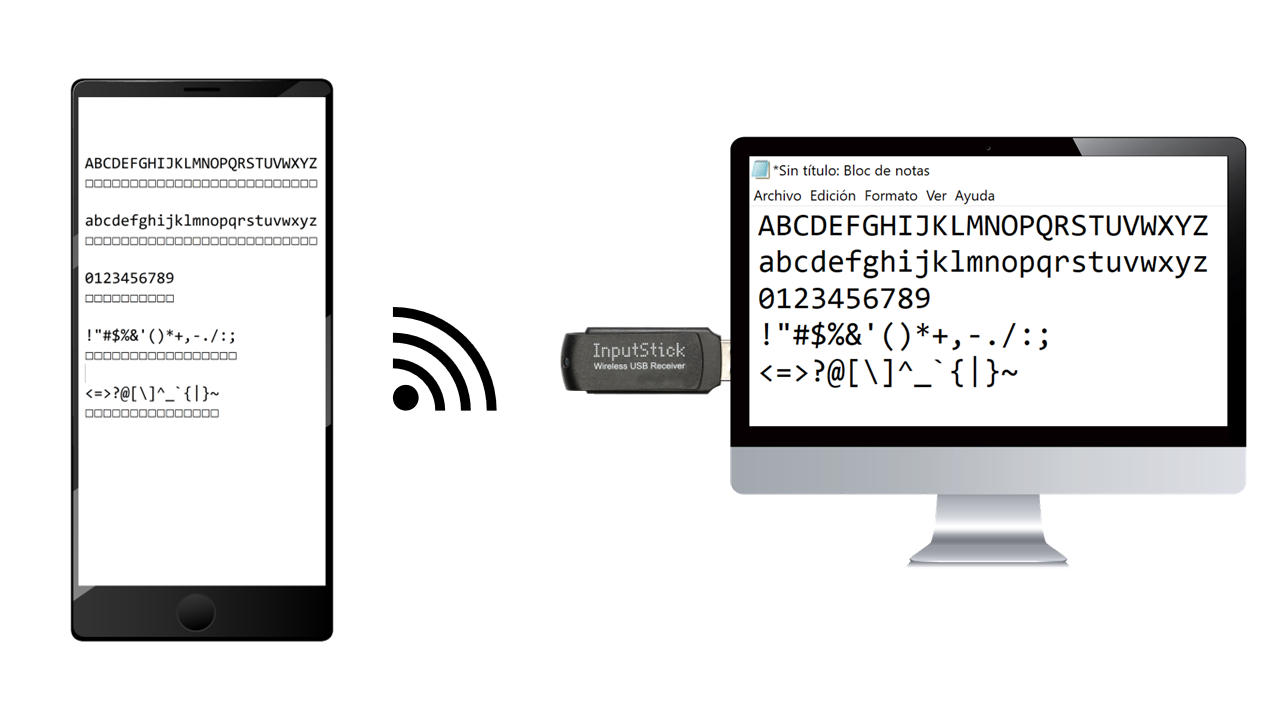
\includegraphics[width=\textwidth]{gfx/diagrama_texto.png}
    \caption{Maqueta de identificación de disposición. Realización propia.}
    \label{fig:diagrama_texto}
    El ordenador sobremesa es a modo de ejemplo, pero es sustituible por cualquier dispositivo compatible con \gls{usb} \gls{hid}.\newline
    Marco de móvil. Imagen por brgfx en Freepik.com.\newline
    Marco de monitor. Imagen por d3images en Freepik.com.\newline
\end{figure}

\end{itemize}